\newpage
\section{RESULTS AND DISCUSSION}

%%%%%%%%%%%%%%%%%%%%%%%%%%%%%%%%%%%%%%%%%%%%%%%%%%%%%%%%%%%%%%%%%%%%%%%%%%%%%%%%%%%%%%%%
%%%%%%%%%%%%%%%%%%%%%%%%%%%%%%%%%%%%%%%%%%%%%%%%%%%%%%%%%%%%%%%%%%%%%%%%%%%%%%%%%%%%%%%%

\subsection{Simulations of API}
The box of neat carbamazepine contained 800 molecules (24~000 atoms), after equilibration run ($T$=500 K), the size of the box was 66 \r{A}. In the naproxen simulation box 800 molecules were presented (24~800 atoms), balanced box size was 66 \r{A}. For ibuprofen the balanced box size with 800 molecules (26~400 atoms) was 67 \r{A}. The simulation box containing 600 molecules (24~600 atoms) of indomethacine had size of 66 \r{A}.

\begin{table}[htb!]
	\caption{Calculated mixing energies and volumes for API mixtures of different concentrations, simulations under 500 K.}
	\centering
	\begin{tabular}{lccc} \toprule
		{\textbf{API}} & {\textbf{\boldmath{$N_{\text{API}}$}}} & \textbf{{\boldmath{$N_{\text{atoms}}$}}} & \textbf{{\boldmath{$l_{\text{box}}$, \AA}}} \\
		\midrule
		carbamazepine  & 800 & 24 000 & 66 \\		
		naproxen  & 800 & 24~800 & 66 \\
		ibuprofen  & 800 & 26~400 & 67 \\
		naproxen  & 600 & 24~600 & 66 \\
		\bottomrule
	\end{tabular}
	\label{tab:API_n} 
\end{table}

COMPARISON OF DENSITIES WITH EXPERIMENTS?

\subsection{Simulations of mixtures of APIs and PLA}
\subsubsection{Calculated properties of mixtures}
Mixing energies and volumes were calculated for both systems, and the comparison is shown in Table \ref{tab:vobjemy}. The data show that a mixture of naproxen and PLA can create a more advantageous arrangement of molecules in space, meaning that the mixing volumes are negative. For carbamazepine the trend is the opposite; this could be caused by the shape of the carbamazepine molecule when the mixture needs more space. From the positive changes in energies, we can assume that mixing the APIs with PLA can reduce the interactions between API-API molecules, and also that new interactions between API and PLA are not developed in order to compensate for the API-API cohesion.  

\begin{table}[htb!]
	\caption{Calculated mixing energies and volumes for API mixtures of different concentrations, simulations under 500 K.}
	\centering
	\begin{tabular}{lSSS} \toprule
		{\textbf{API}} & {\textbf{\boldmath{$x_{\text{API}}$}}} & \textbf{{\boldmath{$V_{\text{m, mixing}}$, cm$^3$/mol}}} & \textbf{{\boldmath{$E_{\text{m, mixing}}$, kJ/mol}}} \\
		\midrule
		carbamazepine  & 0.85 & 0.97 & 4.79 \\
		& 0.92 & 0.48 & 3.17 \\ 
		& 0.95   & 0.21 & 2.68    \\
		\midrule
		naproxen  & 0.85 & -7.07 & 7.50 \\
		& 0.92  & -8.50 & 6.24\\ 
		& 0.95   & -9.85 & 4.75   \\ \bottomrule
	\end{tabular}
	\label{tab:vobjemy} 
\end{table}

\subsubsection{Glass transition temperature}
The glass transition temperatures of the mixtures were evaluated from the simulated annealing simulations by fitting a hyperbola to the temperature-density data. The whole methodology is described in the paper written by Alzate-Vargas\cite{alzate-vargas_uncertainties_2018}, the main equation of the fit is Equation \ref{eq:fit}

\begin{equation}\label{eq:fit}
	\rho(T)=\rho_0-a\left(T-T_0\right)-b\left[\frac{1}{2}\left(T-T_0\right)+\sqrt{\frac{\left(T-T_0\right)^2}{4}+e^c}\right].
\end{equation}

Since this method is sensitive to the initial state of the simulated box, more simulated data starting from different conformations must be provided to evaluate $T_\text{g}$. In this work we used 5 simulations from different initial states.

The resulting value for carbamazepine is $T_{\text{g, cbz}} = 385 \pm 4$ (k = 2) and for naproxen is $T_{\text{g, nap}} = 365 \pm 2$ (k = 2). 

\subsubsection{Radial distribution functions}

Then, all RDFs of mixtures containing the API-API interaction were scaled onto the pure API RDF signal for better visualisation using the following Equation \ref{eq:RDF_formula}

\begin{equation}\label{eq:RDF_formula}
	\text{RDF}_{\text{scaled}} = \text{RDF} \cdot \frac{\displaystyle\frac{V_{\text{API}}}{N_{\text{API}}}}{\displaystyle{\frac{V_{\text{mix}}}{N_{\text{mix}}}}},
\end{equation}

where $V_{\text{API}}$ is the average volume of the pure API simulation box, $N_{\text{API}}$ is the number of molecules in the pure API simulation box and, respectively, for mixtures.

Sampling the radial distribution function from the simulations was done to explore the interactions that are having the highest impact. The hydrogen bonds were mostly studied. All RDF data containing the API-API interaction in the mixtures were scaled for the intensities of the pure API signal. The strongest API-API interaction was chosen and plotted to study the change between simulations with different concentrations of PLA. 

For ibuprofen, the interaction between hydrogen from OH group and oxygen from OC was studied. For naproxen, the hydrogen bonding between two carboxyl groups was studied, for carbamazepine, hydrogen bonding was studied between the N$\text{H}_\text{2}$ and OC group and for indomethacine the interaction of oxygen from OC and hydrogen from OH was studied.  The selected atom types involved in interactions are visualised in Figure \ref{fig:APIs}. 

\begin{figure}[htb!]
	\centering
	\subfloat{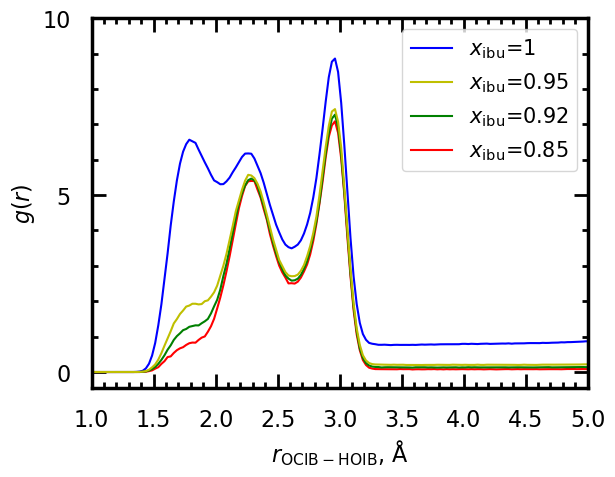
\includegraphics[width=0.4\linewidth]{img/rdf_ibu_s_api_r2.png}}
	%\subfloat{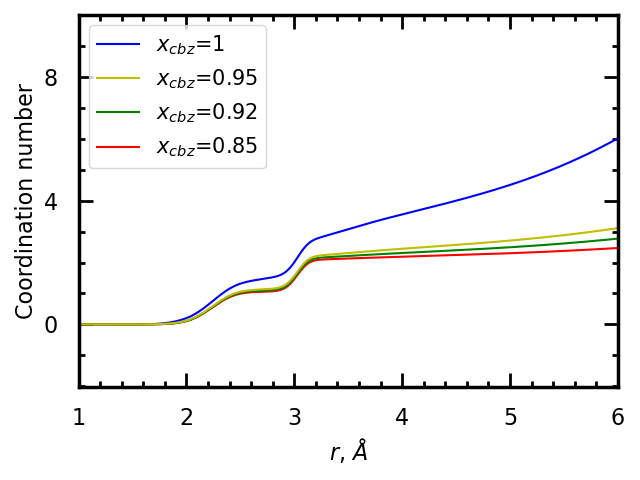
\includegraphics[width=0.4\linewidth]{img/coord_cbz_r2.png}}
	\caption{Radial distribution function of the API-API interaction between HOIB hydrogen atom bonded on oxygen and OCIB oxygen atom in a mixture of ibuprofen and PLA for different concentration normalized on values for pure ibuprofen, temperature of 300~K in the left upper corner and 500~K bottom left, coordination numbers on the right.}
	\label{fig:ibu_s_RDF_}
\end{figure}

The RDF of the selected interaction of naproxen is shown in Figure \ref{fig:nap_RDF_}. Here is the situation very different, the height of the first peak changes for different concentrations of PLA. For the higher concentration of PLA, the occurrence of the two hydrogen bonds carboxyl group contact is less important, and the contact of the groups is made only by one hydrogen bond.

\begin{figure}[htb!]
	\centering
	\subfloat{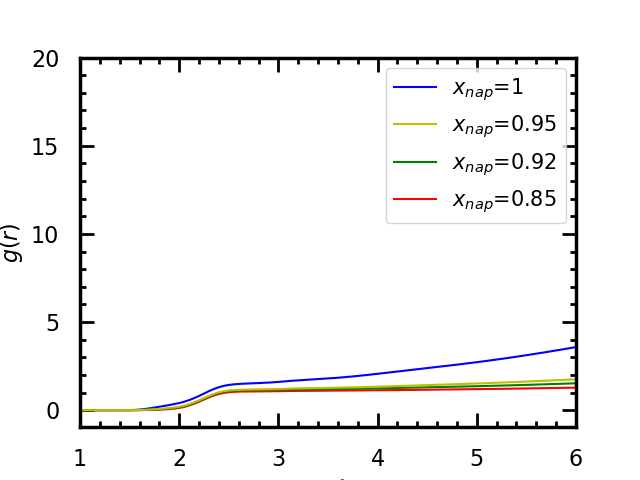
\includegraphics[width=0.4\linewidth]{img/rdf_nap_api_r1.png}}
	\subfloat{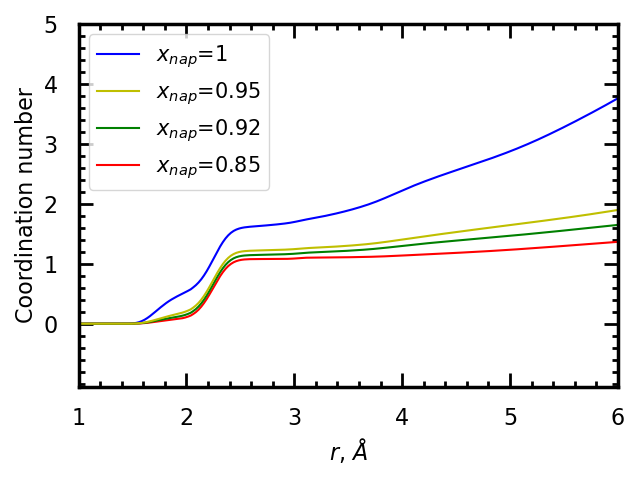
\includegraphics[width=0.4\linewidth]{img/coord_nap_r1.png}}\\
	\subfloat{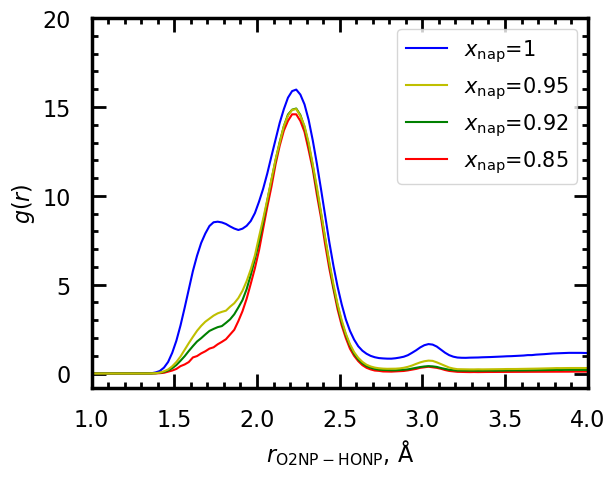
\includegraphics[width=0.4\linewidth]{img/rdf_nap_api_r2.png}}
	\subfloat{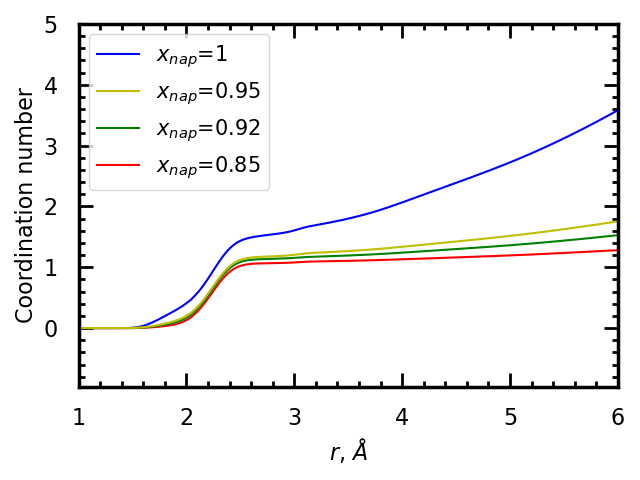
\includegraphics[width=0.4\linewidth]{img/coord_nap_r2.png}}
	\caption{Radial distribution function of the API-API interaction between HONP hydrogen atom and O2NP oxygen atom from COOH group in a mixture of naproxen and PLA for different concentration normalized on values for pure naproxen, temperature of 300~K in the left upper corner and 500~K bottom left, coordination numbers on the right.}
	\label{fig:nap_RDF_}
\end{figure}

The RDF of the hydrogen bonding interaction of carbamazepine is shown in Figure \ref{fig:cbz_RDF_}. The shape and signal response of the peaks for the mixtures are similar for both temperatures, meaning that the impact of the concentration of PLA on the cohesion of carbamazepine in the mixture is very low. 

\begin{figure}[htb!]
	\centering
	\subfloat{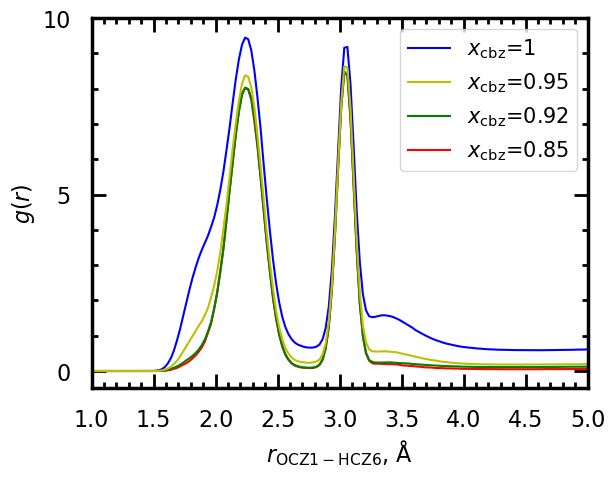
\includegraphics[width=0.4\linewidth]{img/rdf_cbz_api_r1.png}}
	\subfloat{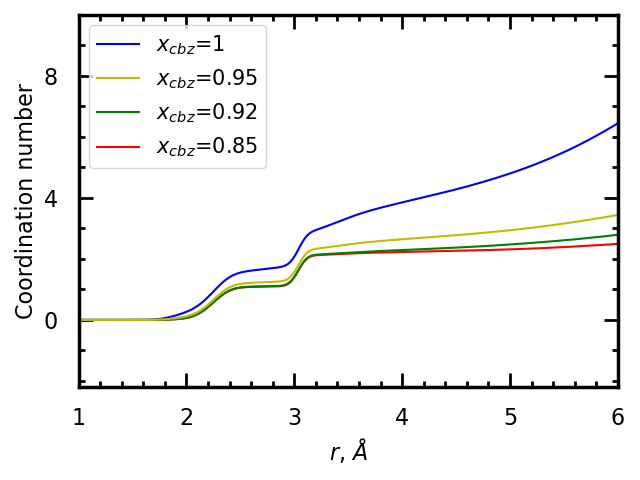
\includegraphics[width=0.4\linewidth]{img/coord_cbz_r1.png}}\\
	\subfloat{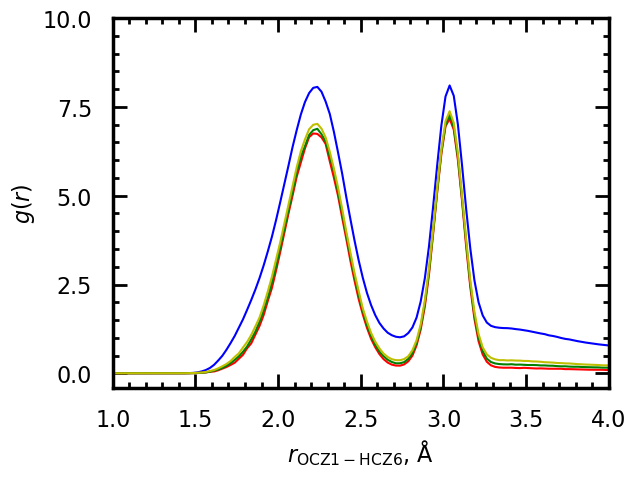
\includegraphics[width=0.4\linewidth]{img/rdf_cbz_api_r2.png}}
	\subfloat{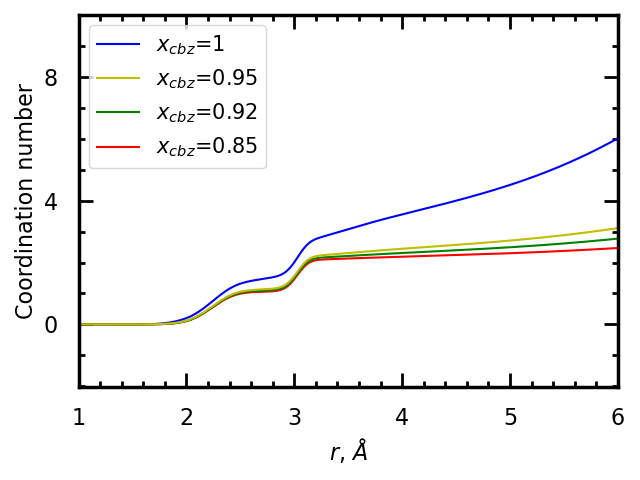
\includegraphics[width=0.4\linewidth]{img/coord_cbz_r2.png}}
	\caption{Radial distribution function of the API-API interaction between HCZ6 hydrogen atom bonded on nitrogen and OCZ1 oxygen atom in a mixture of carbamazepine and PLA for different concentration normalized on values for pure carbamazepine, temperature of 300~K in the left upper corner and 500~K bottom left, coordination numbers on the right.}
	\label{fig:cbz_RDF_}
\end{figure}



\begin{figure}[htb!]
	\centering
	\subfloat{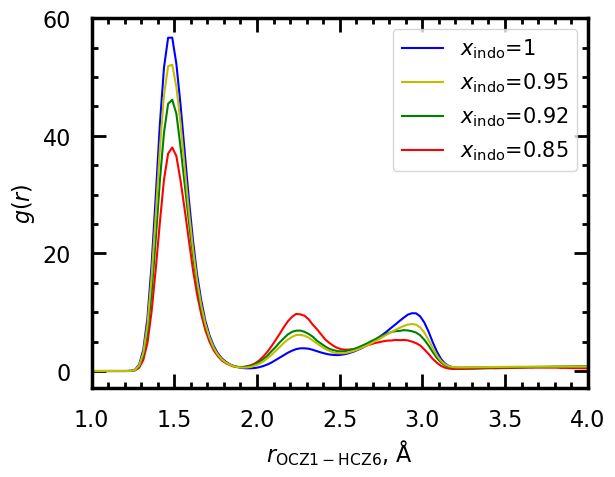
\includegraphics[width=0.4\linewidth]{img/rdf_indo_api_r1.png}}\\
	%\subfloat{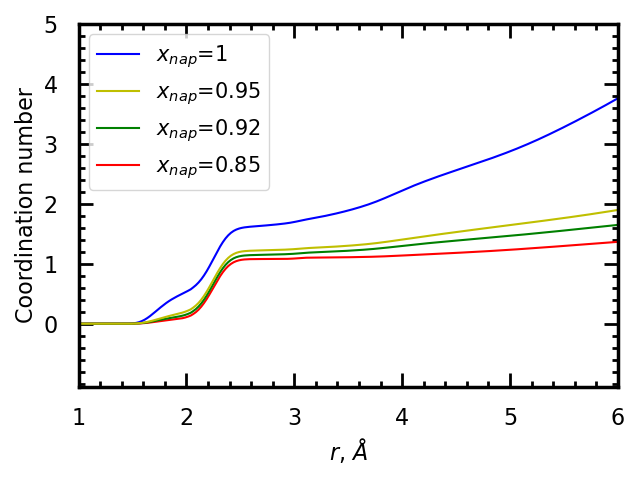
\includegraphics[width=0.4\linewidth]{img/coord_nap_r1.png}}\\
	\subfloat{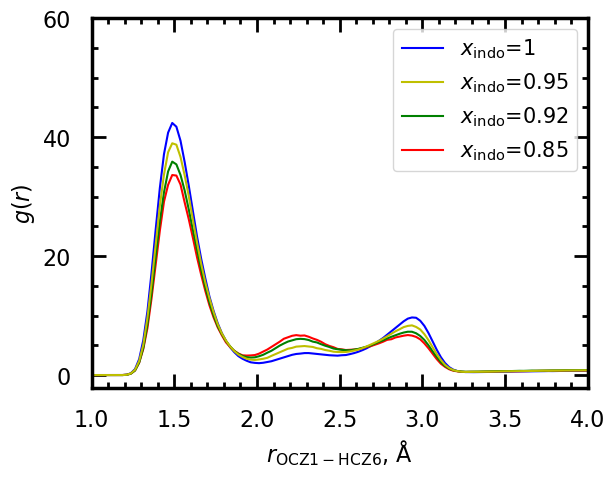
\includegraphics[width=0.4\linewidth]{img/rdf_indo_api_r2.png}}\\
	%\subfloat{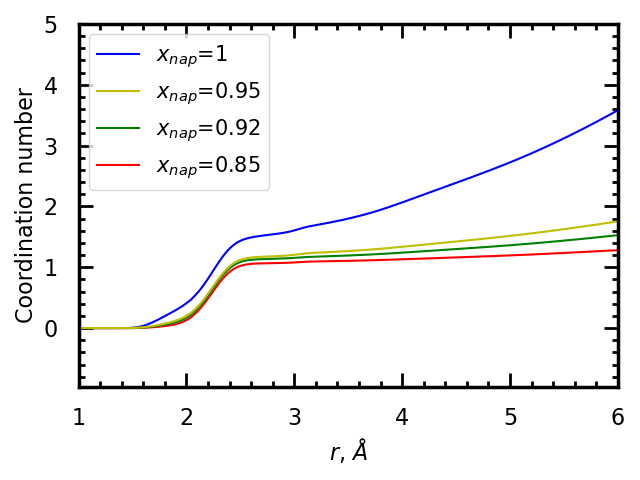
\includegraphics[width=0.4\linewidth]{img/coord_nap_r2.png}}
	\caption{Radial distribution function of the API-API interaction between HCZ6 hydrogen atom and OCZ1 oxygen atom from COOH group in a mixture of indomthacine and PLA for different concentration normalized on values for pure indomethacine, temperature of 300~K in the left upper corner and 500~K bottom left, coordination numbers on the right.}
	\label{fig:nap_RDF_}
\end{figure}




The hydrogen bonding between API and PLA was also studied. The contact visualization is available in Figure \ref{fig:contact}.

\begin{figure}[htb]
	\begin{subfigure}{0.33\textwidth}
		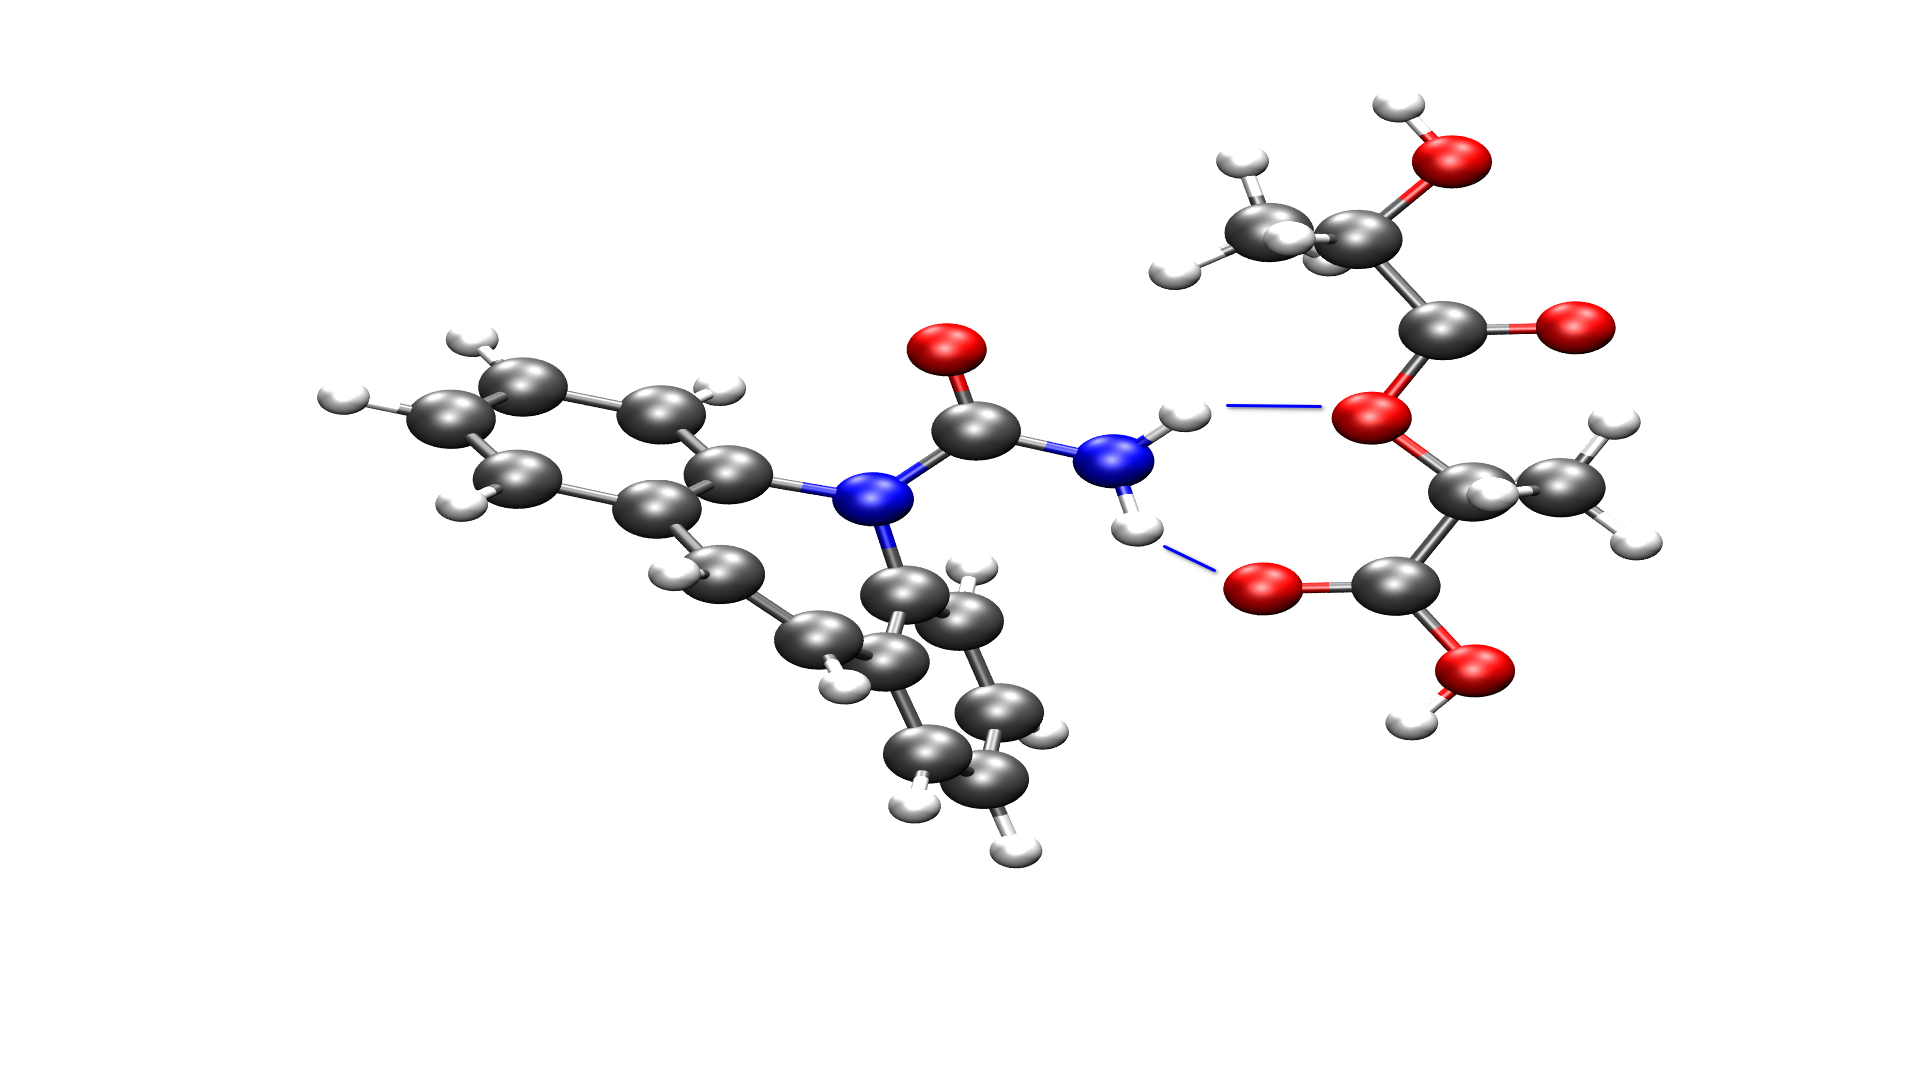
\includegraphics[width=\linewidth]{img/cbz_interakce.png} 
	\end{subfigure}
	\begin{subfigure}{0.31\textwidth}
		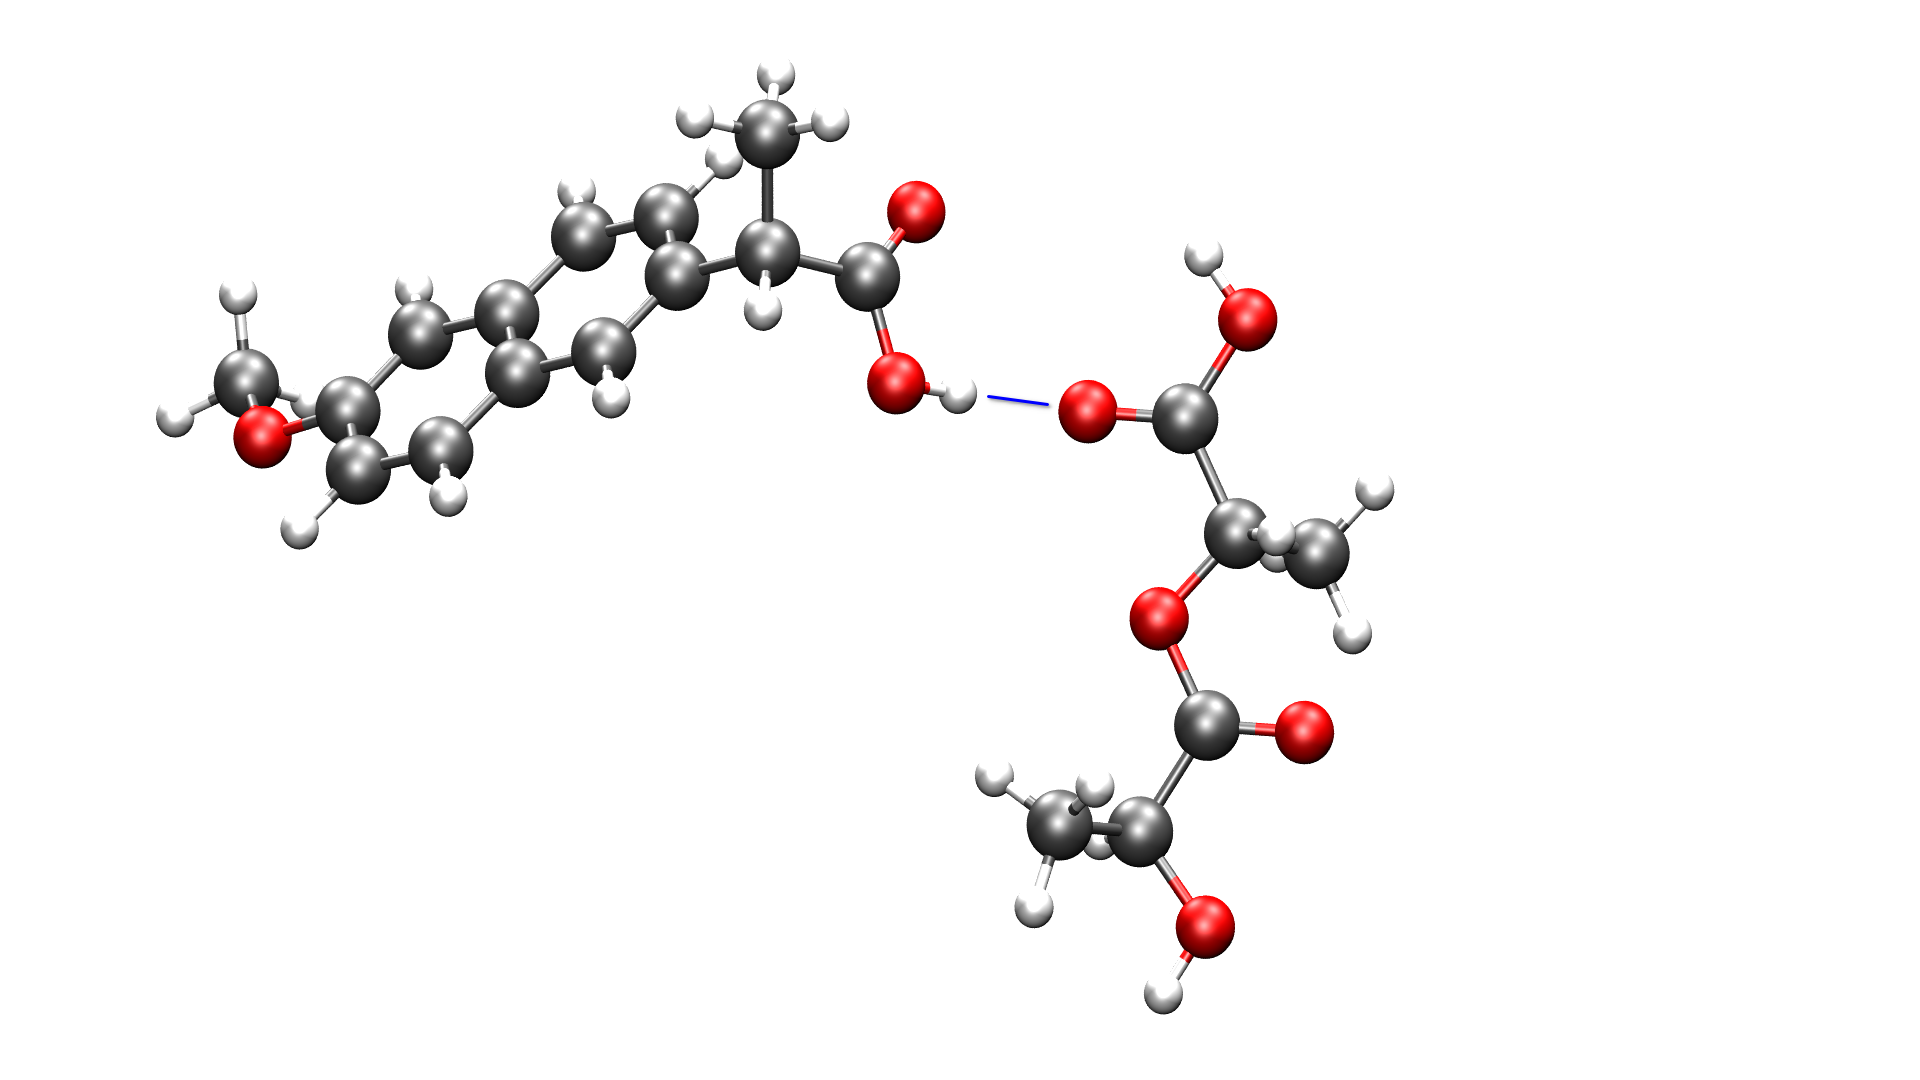
\includegraphics[width=\linewidth]{img/nap1_interakce.png} 
	\end{subfigure}   	
	\begin{subfigure}{0.33\textwidth}
		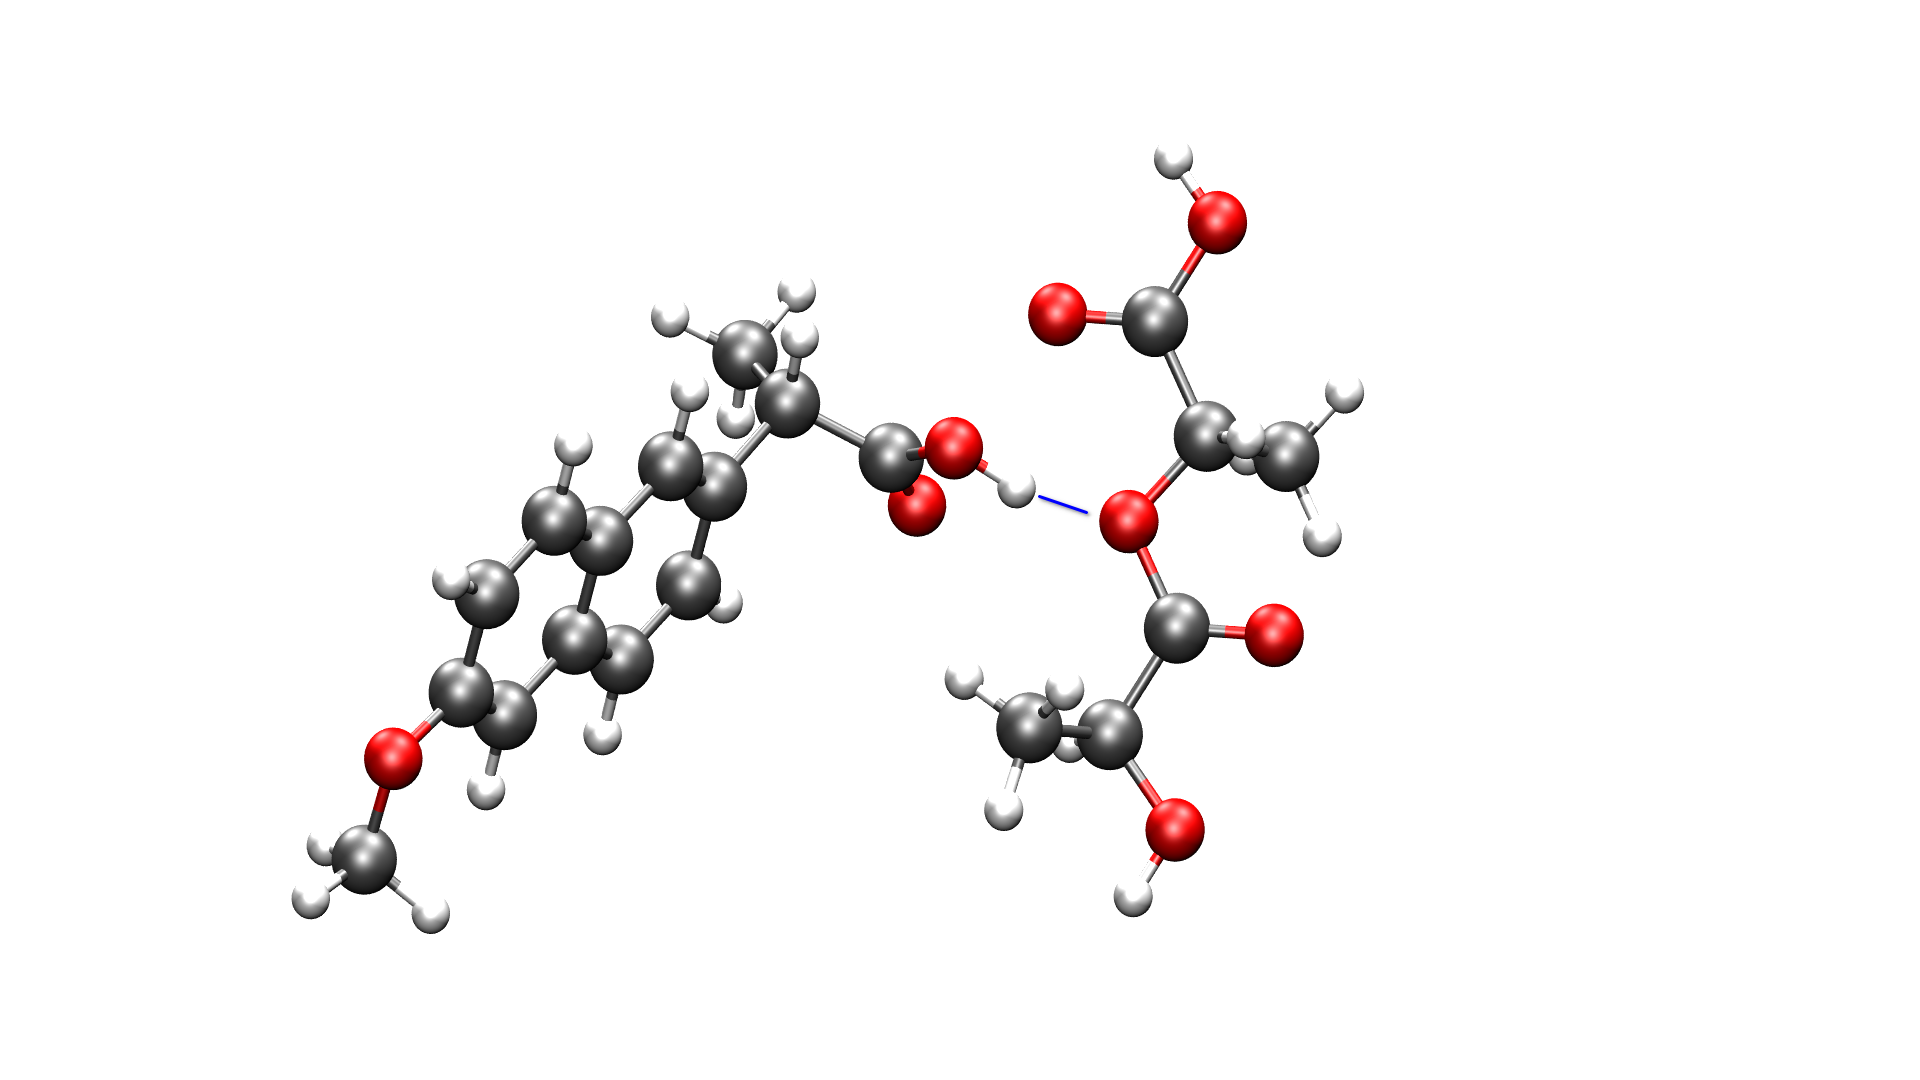
\includegraphics[width=\linewidth]{img/nap2_interakce.png} 
	\end{subfigure}
	\caption{Visualization of studied interactions of PLA-API, for carbamazepine on the left and for naproxen on the right.}
	\label{fig:contact}    
\end{figure}


The RDF of hydrogen bonding with the carbonyl group is shown in Figure \ref{fig:carbonyl}. For carbamazepine, those interactions are weak, we can see that the intensity of the first peak is really low. Under temperature 300 K slightly above one, but for 500 K the peak is below one, meaning that this interaction occurs less at a small distance than in the rest of the system. The value converges to one in a long distance. For naproxen, the interaction is more relevant, and the intensity of the peak is much higher but still less than in the NAP-NAP interactions.

\newpage
\begin{figure}[]
	\centering
	\subfloat{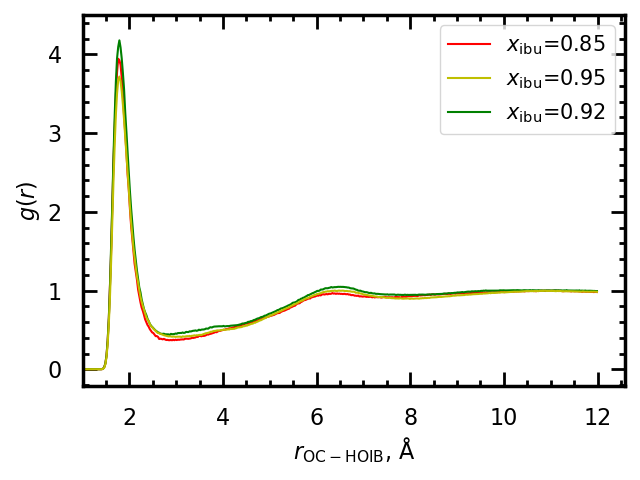
\includegraphics[width=0.5\linewidth]{img/RDF_ibu_s_20_2.png}}
	\subfloat{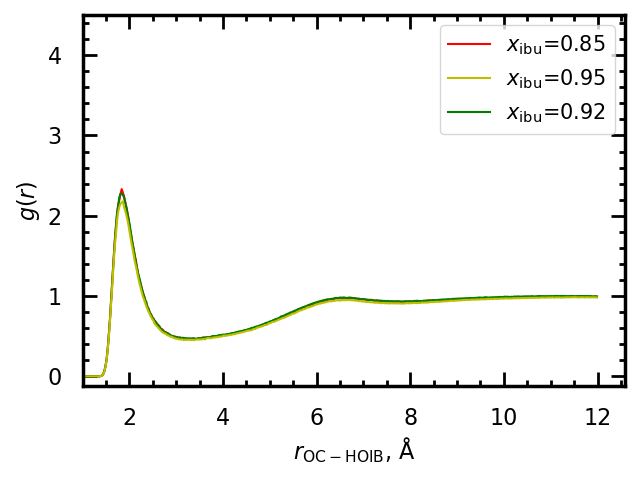
\includegraphics[width=0.5\linewidth]{img/RDF_ibu_s_20_2_r2.png}}\\
	\vspace{-0.2cm}
	\subfloat{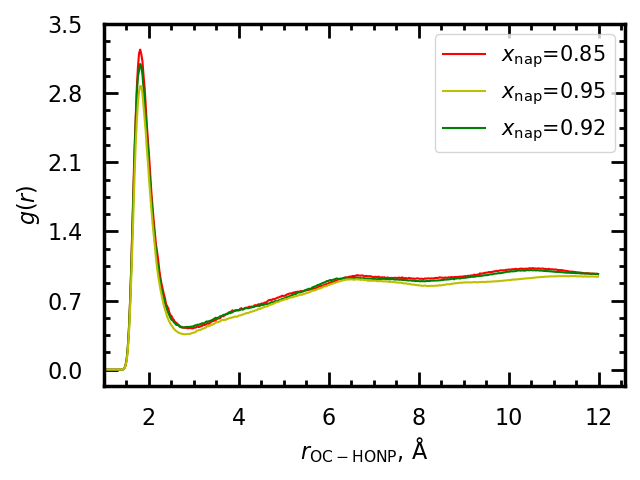
\includegraphics[width=0.5\linewidth]{img/RDF_nap_2_31.png}}
	\subfloat{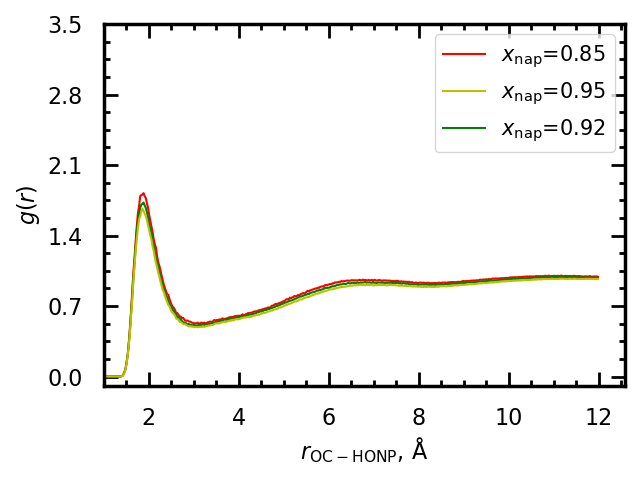
\includegraphics[width=0.5\linewidth]{img/RDF_nap_2_31_r2.png}}\\
	\vspace{-0.2cm}
	\subfloat{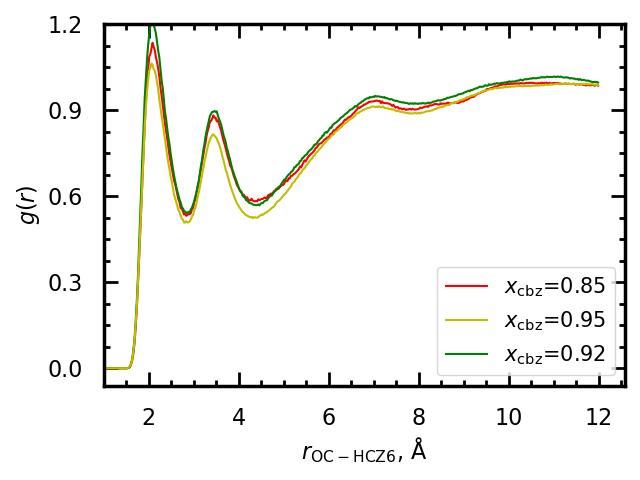
\includegraphics[width=0.5\linewidth]{img/RDF_cbz_2_27.png}}
	\subfloat{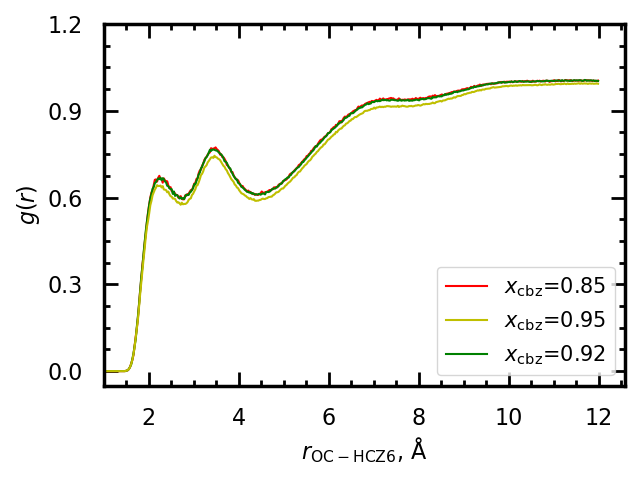
\includegraphics[width=0.5\linewidth]{img/RDF_cbz_2_27_r2.png}}\\
	\vspace{-0.2cm}
	\subfloat{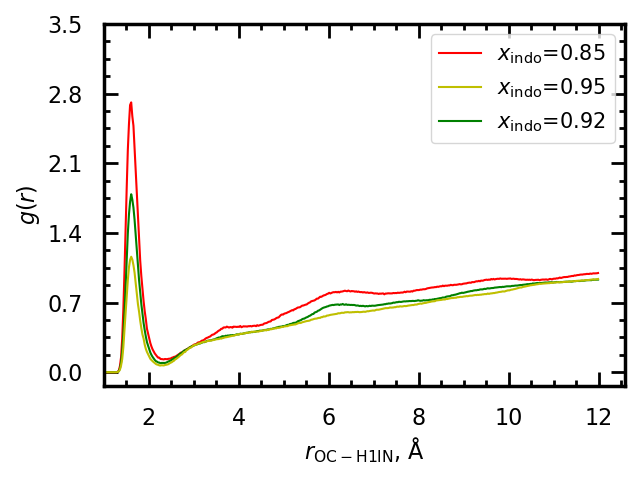
\includegraphics[width=0.5\linewidth]{img/RDF_indo_2_36.png}}
	\subfloat{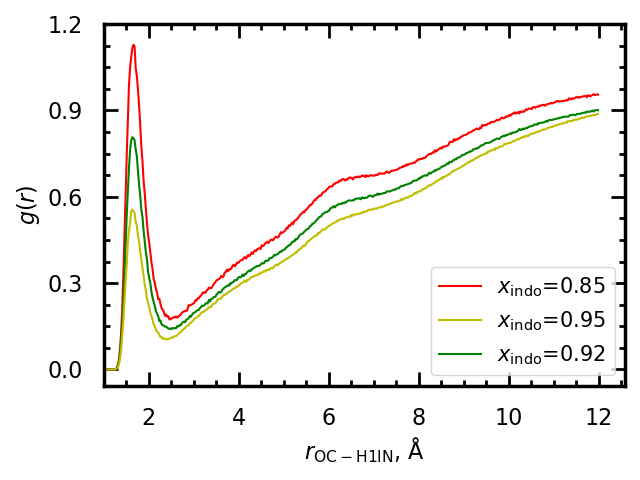
\includegraphics[width=0.5\linewidth]{img/RDF_indo_2_36_r2.png}}
		\vspace{-0.2cm}
	\caption{Radial distribution function of the interaction between hydrogen atoms and oxygen atom from carbonyl group in PLA, first ibuprofen on top, second naproxen, third carbamazepine and indomethacine in the bottom, temperature 300~K on the left and 500~K on the right.}
	\label{fig:carbonyl}
\end{figure}

The hydrogen bonds with the oxygen bonded by ether bond in PLA are shown in Figure \ref{fig:ether}. Here is the same situation as in the previous contact with carbonyl oxygen, but for naproxen, the interaction is less relevant. Both values also converge to 1 in a long distance.

\vspace{-0.5cm}
\begin{figure}[H]
	\centering
	\subfloat{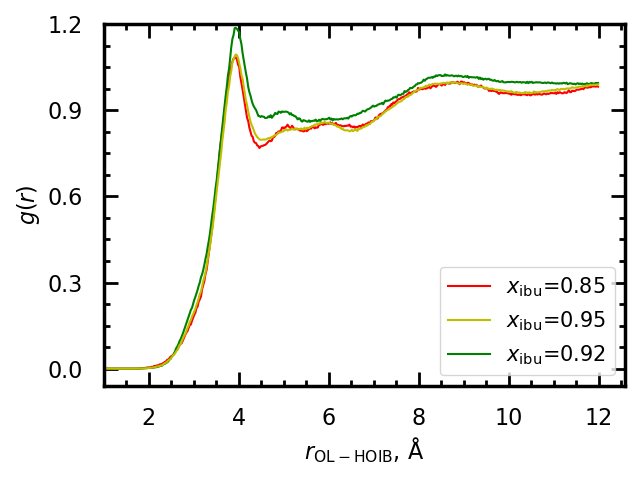
\includegraphics[width=0.5\linewidth]{img/RDF_ibu_s_20_6.png}}
	\subfloat{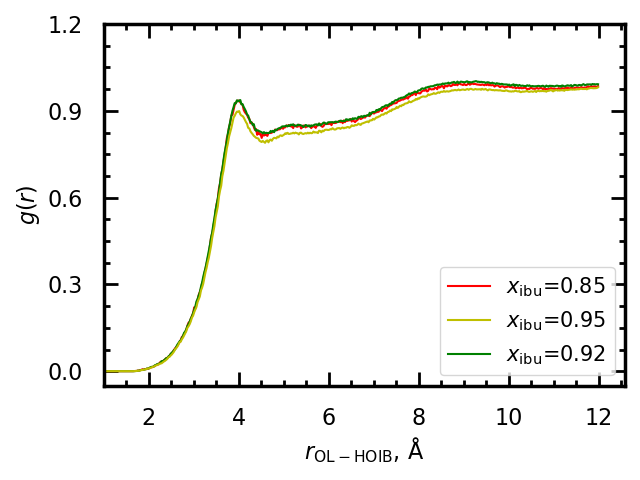
\includegraphics[width=0.5\linewidth]{img/RDF_ibu_s_20_6_r2.png}}\\
	\vspace{-0.2cm}
	\subfloat{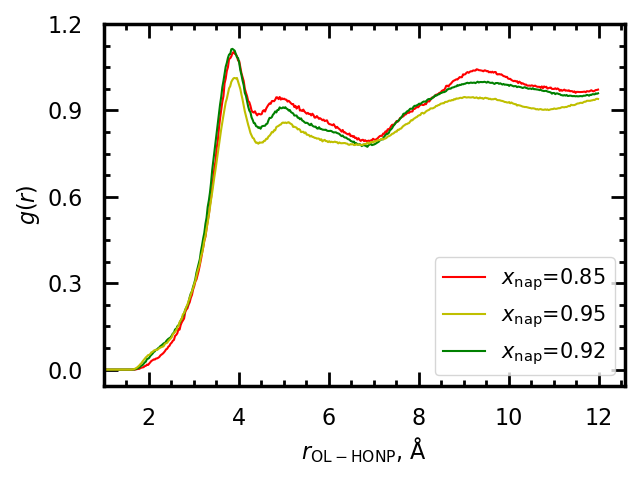
\includegraphics[width=0.5\linewidth]{img/RDF_nap_6_31.png}}
	\subfloat{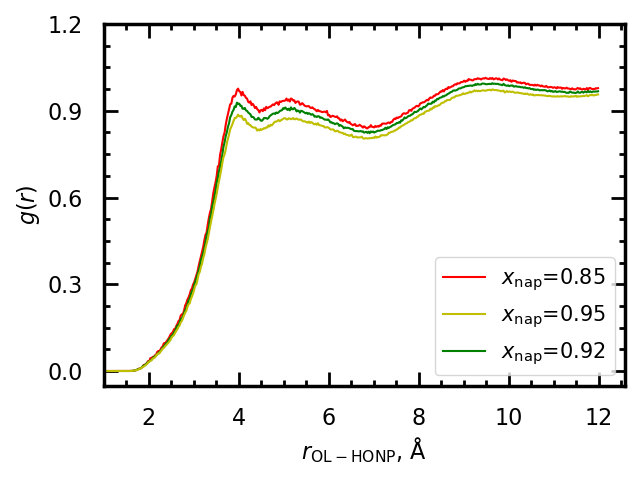
\includegraphics[width=0.5\linewidth]{img/RDF_nap_6_31_r2.png}}\\
	\vspace{-0.2cm}
	\subfloat{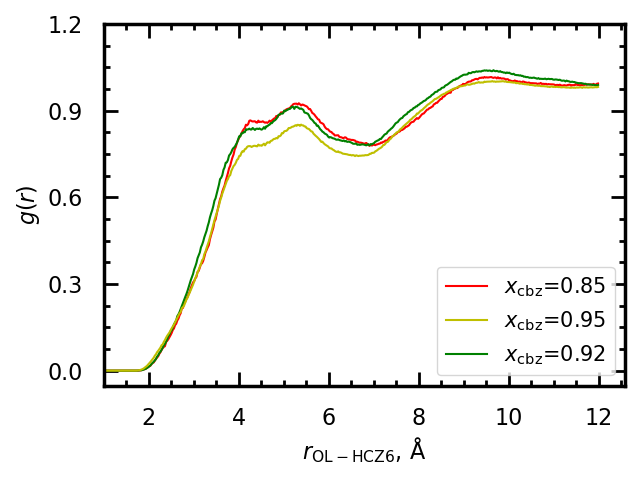
\includegraphics[width=0.5\linewidth]{img/RDF_cbz_6_27.png}}
	\subfloat{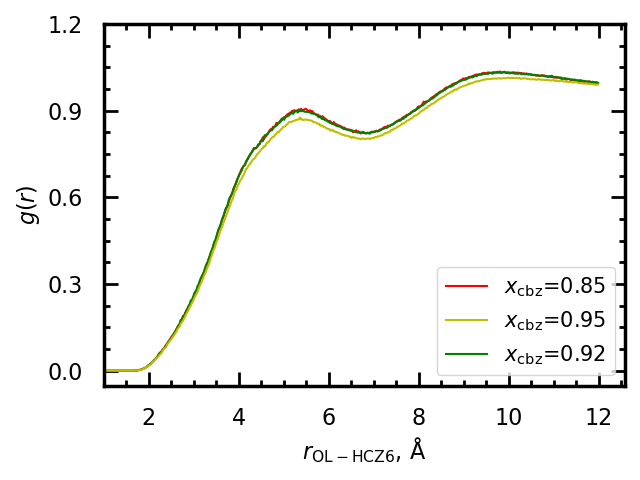
\includegraphics[width=0.5\linewidth]{img/RDF_cbz_6_27_r2.png}}\\
	\vspace{-0.2cm}
	\subfloat{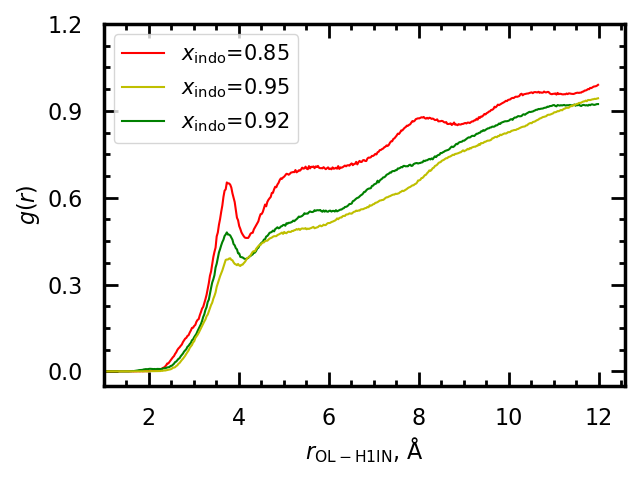
\includegraphics[width=0.5\linewidth]{img/RDF_indo_36_6.png}}
	\subfloat{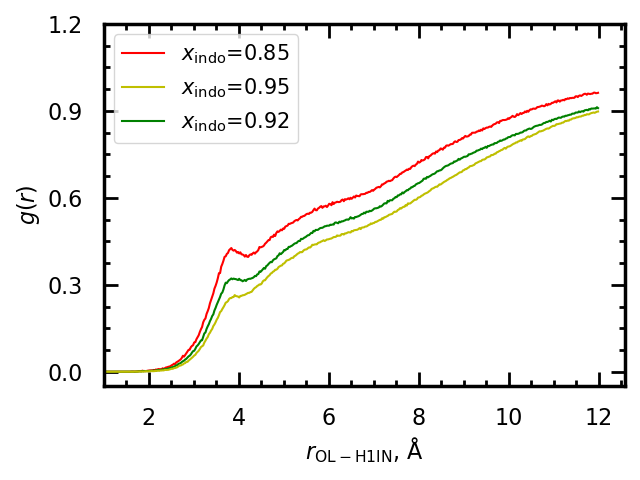
\includegraphics[width=0.5\linewidth]{img/RDF_indo_36_6_r2.png}}
	\vspace{-0.2cm}
	\caption{Radial distribution function of the interaction between hydrogen atoms and oxygen atom bonded by ether bond in PLA, first ibuprofen on top, second naproxen, third carbamazepine and indomethacine in the bottom, temperature 300~K on the left and 500~K on the right.}
	\label{fig:ether}
\end{figure}

\subsubsection{Diffusion coefficients}
The MSDs were sampled from the 10~ns long run simulations every 1000 fs (integration step 1 fs). At each sampled time step, obtained MSD data were averaged over all API molecules and then plotted as a function of simulation time. The MSD dependencies were then interpolated by a linear functions and related self-diffusivities of the API in the mixtures were evaluated from the slope of the line using the following Equation \ref{eq:D}

\begin{equation}\label{eq:D}
	D_{\text{API}} = \frac{a}{2d}, 
\end{equation}
where $D$ is the diffusion coefficient, $a$ is the slope of the line and $d$ is the dimensionality of the trajectory (3 in our case).

The MSD data for APIs in mixtures with PLA for $T$=500~K are plotted in Figure \ref{fig:msd_r2}. For ibuprofen, there is a significant difference between mobility of neat API and API mixed within the polymer. This could be result of very strong API-PLA interaction forming in the mixture. The data of carbamazepine shows that with increasing API concentration, mobility also increases. There is also not that enormous difference between neat API. For naproxen, it seems that there is no change for different concentrations of mixtures, also in neat API the mobility is higher. The situation for indometacine is completely different. For neat API the mobility is really low compared to mixtures with PLA. This behaviour seems strange, the reason could be, that in pure API, there are really strong API-API interactions that decrease the mobility. Also the MSD values are much lower.

\begin{figure}[htb]
	\centering
	\subfloat{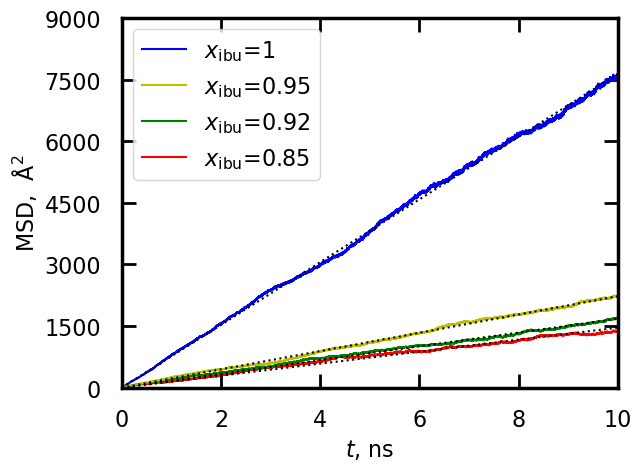
\includegraphics[width=0.4\linewidth]{img/msd_ibu_s_api_r2.png}}
	\subfloat{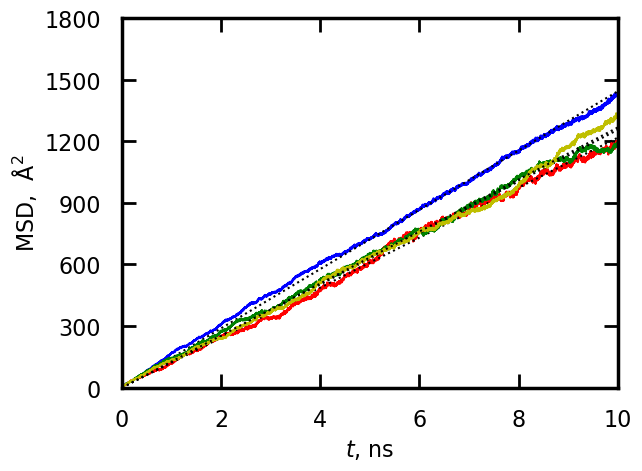
\includegraphics[width=0.4\linewidth]{img/msd_nap_api_r2.png}}\\
	\subfloat{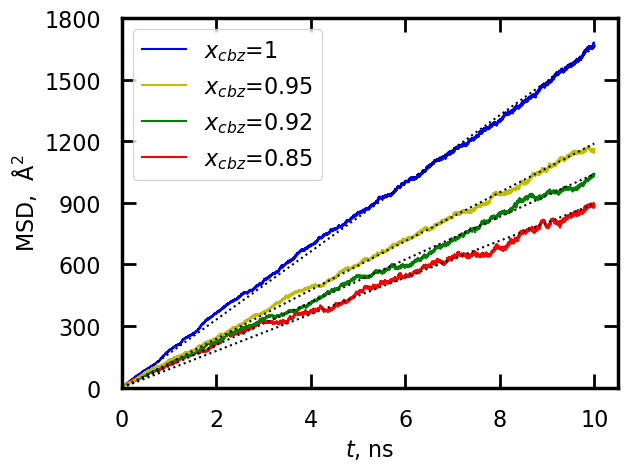
\includegraphics[width=0.4\linewidth]{img/msd_cbz_api_r2.png}}
	\subfloat{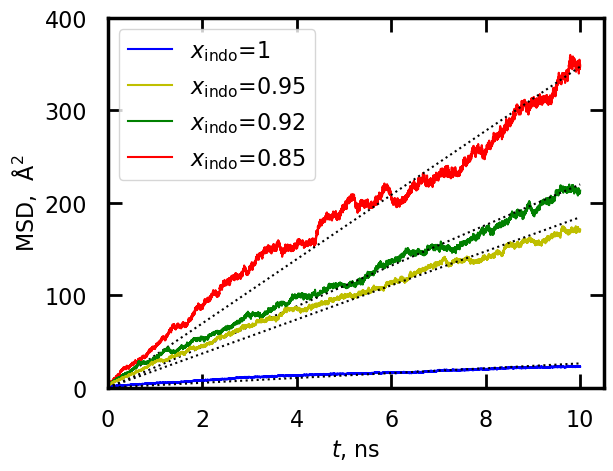
\includegraphics[width=0.4\linewidth]{img/msd_indo_api_r2.png}} 
	\caption{MSD from simulations under 500 K, ibuprofen (\textbf{top left}), naproxen (\textbf{top right}), carbamazepine (\textbf{bottom left}) and indomethacin (\textbf{bottom right}).}
	\label{fig:msd_r2}    
\end{figure}

\newpage
Self-diffusivities were evaluated from the above data and plotted in Figure \ref{fig:d}. The data reveal that in pure liquid carbamazepine the diffusion is faster than in naproxen. For higher temperatures, the main factor affecting diffusion is the shape of the molecules, not the strength of the intermolecular interactions. This is caused because the kinetic energy is higher than the potential for higher temperatures.
\begin{figure}[htb!]
	\centering
	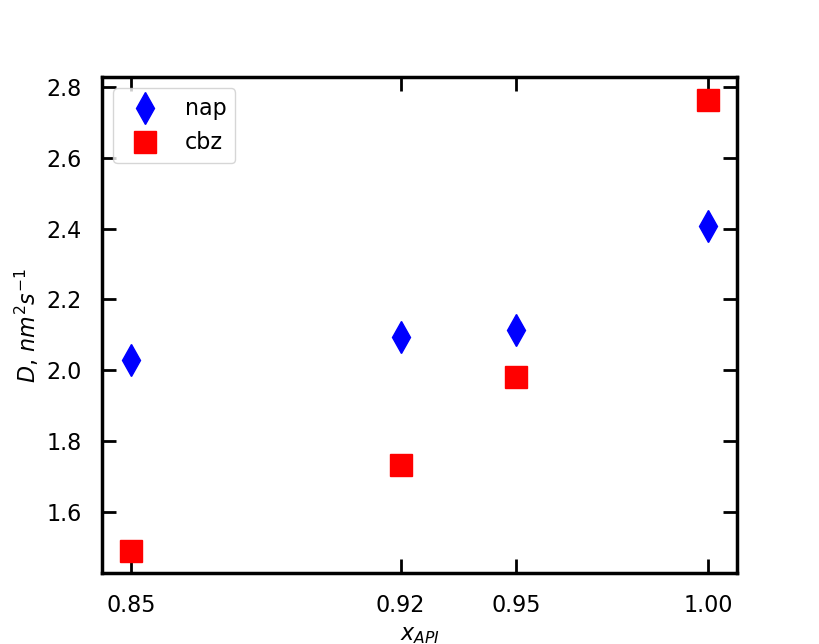
\includegraphics[width=0.4\linewidth]{img/d_coeficienty.png} 
	\caption{Self-diffusivities for carbamazepine and naproxen as a function of their concentration in the mixtures, temperature 500 K.}
	\label{fig:d}    
\end{figure}  

MSD was also evaluated at a lower temperature of 300 K, Figure \ref{fig:msd_r1}. There is the opposite trend. From these data sets, we can assume that carbamazepine has lower interactions with polymer because the mobility in the mixtures is higher than that in the pure state. The mobility of naproxen is always lower in mixtures, which is related to its stronger interactions with the polymer. The strength of the intermolecular interactions has a greater impact, meaning that paired molecules NAP-API slow the diffusion of other particles.

\begin{figure}[htb]
	\centering
	\subfloat{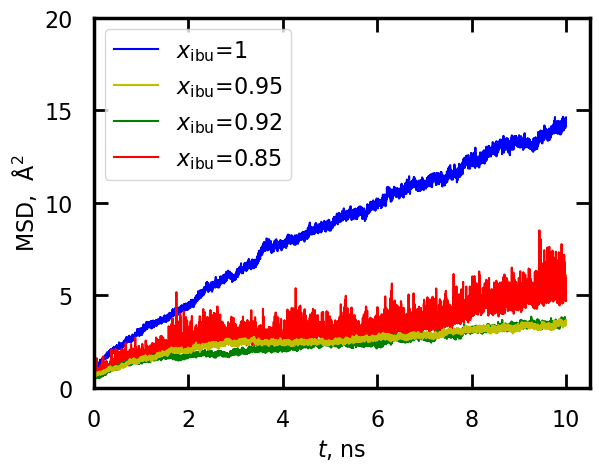
\includegraphics[width=0.4\linewidth]{img/msd_ibu_s_api_r1.png}}
	\subfloat{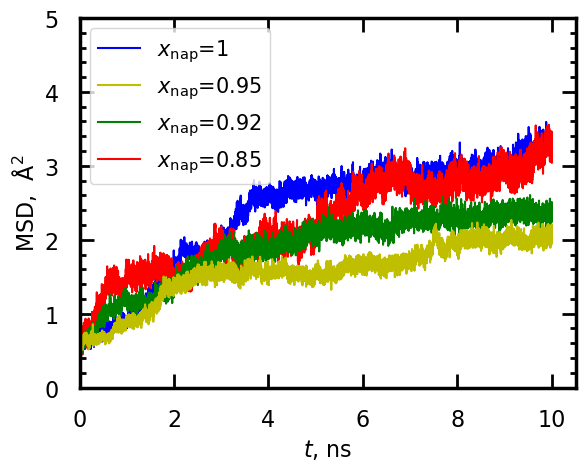
\includegraphics[width=0.4\linewidth]{img/msd_nap_api_r1.png}}\\
	\subfloat{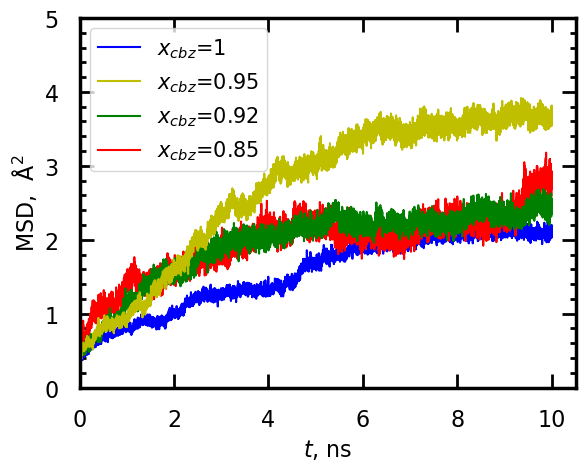
\includegraphics[width=0.4\linewidth]{img/msd_cbz_api_r1.png}}
	\subfloat{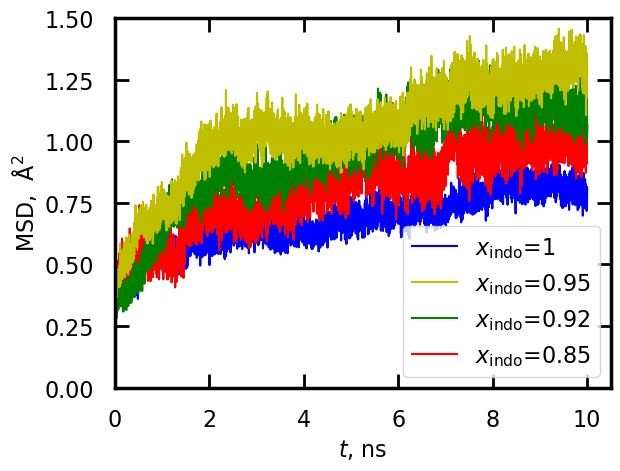
\includegraphics[width=0.4\linewidth]{img/msd_indo_api_r1.png}} 
	\caption{MSD from simulations under 300 K, ibuprofen (\textbf{top left}), naproxen (\textbf{top right}), carbamazepine (\textbf{bottom left}) and indomethacin (\textbf{bottom right}).}
	\label{fig:msd_r1}    
\end{figure}

\subsection{Smesi s polarizovanym polem}

